\documentclass{article}
\usepackage{amsmath,amssymb}
\usepackage{graphicx}
\usepackage{booktabs}
\usepackage{algorithm}
\usepackage{algorithmic}
\usepackage{float}

\title{Accelerating IAPWS-IF97 Formula Evaluation via Recurrence Polynomial-Derivative Computation and Loop Tiling}

\author{Maohua Cheng \\
  School of Energy and Environment, Southeast University \\
  Nanjing 210096, China \\
  \texttt{cmh@seu.edu.cn}}

\date{}

\begin{document}

\maketitle

\begin{abstract}
This paper presents two acceleration techniques for the IAPWS-IF97 industrial formulation for thermodynamic properties of water and steam: recurrence polynomial-derivative computation and loop tiling. Unlike alternative methods such as TTSE and SBTL that avoid direct formula evaluation and support limited input parameter pairs, the proposed techniques directly accelerate the IAPWS-IF97 formula evaluation while maintaining full accuracy and supporting all 12 input parameter pairs. Recurrence polynomial-derivative computation exploits the mathematical relationship between Gibbs/Helmholtz free energy polynomials and their partial derivatives to compute them simultaneously in a single pass, eliminating redundant calculations. Loop tiling partitions polynomial summation into cache-friendly tiles that enable effective SIMD vectorization. Benchmark results demonstrate that the proposed methods achieve 5x to 20x speedup compared to direct implementations. A Rust-based software package, SEUIF97, implements these techniques and supports 36 thermodynamic, transport, and derived properties.
\end{abstract}

\section{Introduction}

The IAPWS-IF97 formulation [1] is the international standard for calculating thermodynamic properties of water and steam. Since its release, it has become the de facto standard in power engineering, process simulation, and thermal system analysis [2]. High-performance computing scenarios such as real-time simulation, optimization, and large-scale model training require fast and accurate water/steam property calculations to meet demanding computational requirements.

The core computational work of IF97 consists of evaluations of Gibbs and Helmholtz free energy polynomials and their partial derivatives, which can become a bottleneck in large-scale simulations requiring millions of property calculations. Since the fundamental form of IF97 equations is based on polynomials with integer exponents and their partial derivatives, achieving fast property calculations fundamentally requires designing efficient evaluation methods for these polynomials. This creates a critical need for optimization techniques that can accelerate such polynomial computations without sacrificing accuracy.

Existing approaches to improving IAPWS-IF97 computational speed fall into two categories. The first category uses alternative formulations that avoid direct polynomial evaluation. IAPWS has proposed the TTSE (Tabular Taylor Series Expansion) [3] and SBTL (Spline-Based Table Lookup) [4] methods, which use precomputed tables with interpolation to achieve fast lookups. However, these methods do not directly evaluate the IF97 formulas, have limited applicability to specific input parameter pairs, and require additional memory for table storage. The second category directly evaluates the IF97 formulas but with limited optimization. Among open-source implementations, freeSteam [5] has applied the repeated squaring method in its C implementation to optimize integer power computation. Most other implementations, including widely used libraries, directly evaluate the formulas term by term without exploiting the polynomial structure for acceleration.

Despite these efforts, significant opportunities for optimization remain unexplored: (1) the recurrence relationship between polynomial terms and their derivatives has not been exploited to eliminate redundant calculations; (2) loop tiling for improving cache locality in polynomial evaluation has not been applied in the IF97 context; and (3) no existing implementation systematically combines multiple optimization techniques while maintaining full formula accuracy and support for all input parameter pairs.

This paper proposes two acceleration techniques that directly accelerate the IAPWS-IF97 formula evaluation:
\begin{enumerate}
    \item \textbf{Recurrence polynomial-derivative computation}: Computing polynomials and their partial derivatives simultaneously in a single pass to eliminate redundant calculations
    \item \textbf{Loop tiling}: Splitting single loops into cache-friendly tiles to improve cache locality and SIMD vectorization
\end{enumerate}

The paper is organized as follows: Section 2 provides an overview of the IAPWS-IF97 formulation and its key characteristics; Section 3 details the acceleration techniques; Section 4 presents comprehensive benchmark results; Section 5 describes the software implementation; and Section 6 concludes the paper.

\section{IAPWS-IF97 Formulation Overview}

The IAPWS-IF97 (International Association for the Properties of Water and Steam, Industrial Formulation 1997) [1] divides the thermodynamic phase diagram of water and steam into five regions, as shown in Figure \ref{fig:if97_regions}. The original 1997 release replaced the corresponding release of 1967 (IFC-67). The 2007 revision extended Region 5 to 50 MPa, and the 2012 consolidated release (R7-97(2012)) is the current standard. This release has been supplemented by additional ``backward'' equations for $p(h,s)$ in Regions 1 and 2, $T(p,h)$, $v(p,h)$, $T(p,s)$, $v(p,s)$ in Region 3, $p(h,s)$ in Region 3 with auxiliary equations for independent variables $h$ and $s$, and $v(p,T)$ in Region 3.

\begin{figure}[htbp]
\centering
\caption{IAPWS-IF97 thermodynamic regions in the pressure-temperature plane}
\label{fig:if97_regions}
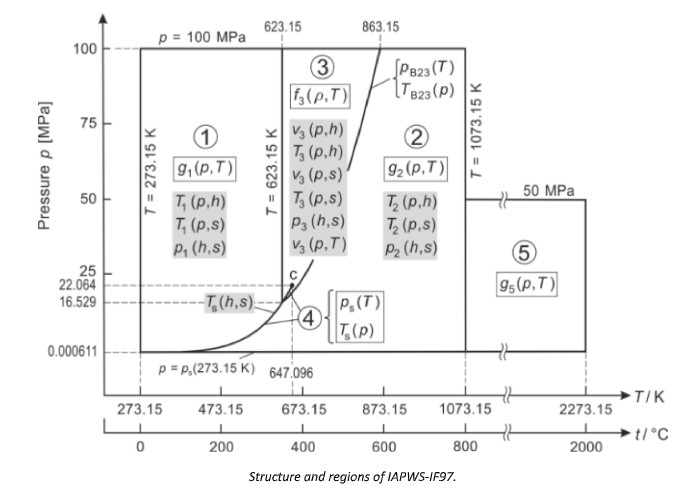
\includegraphics[width=0.85\textwidth]{IAWPS-IF97.jpg}
\end{figure}

In addition, the IAPWS-IF97 Supplementary Release [6] extends the original standard with formulations for:
\begin{itemize}
    \item Transport properties: dynamic viscosity $\mu$ and thermal conductivity $\lambda$
    \item Additional thermodynamic properties: isothermal compressibility $\kappa_T$, isobaric thermal expansion coefficient $\alpha_p$, and specific heat ratio $c_p/c_v$
\end{itemize}

\subsection{Basic Equations}

The core of IAPWS-IF97 consists of two types of fundamental equations, each optimized for specific thermodynamic regions for Regions 1, 2, 3     and 5:

Region 4 (saturation line) provides explicit equations for saturation pressure $p_s(T)$ and saturation temperature $T_s(p)$:

\subsubsection{Gibbs Free Energy Equation (Regions 1, 2, 5)}

Regions 1 (compressed liquid), 2 (superheated vapor), and 5 (high-temperature steam) use the dimensionless Gibbs free energy $g/(RT)$ as the fundamental equation:

\begin{equation}
\frac{g(p,T)}{RT} = \gamma(\pi,\tau) = \sum_{i=1}^{N} n_i \, \pi^{I_i} \, \tau^{J_i}
\label{eq:gibbs}
\end{equation}

where the reduced variables are defined as $\pi = p/p^{*}$ and $\tau = T^{*}/T$, with region-specific scaling parameters $p^{*}$ and $T^{*}$. The coefficients $n_i$ and exponents $I_i$, $J_i$ are provided in tabular form for each region. Table \ref{tab:region_params} summarizes the scaling parameters and number of terms for each Gibbs-based region.

\subsubsection{Helmholtz Free Energy Equation (Region 3)}

Region 3 (near-critical region) uses the dimensionless Helmholtz free energy $f/(RT)$ as the fundamental equation, with density $\rho$ and temperature $T$ as independent variables:

\begin{equation}
\frac{f(\rho,T)}{RT} = \alpha(\delta,\tau) = \alpha^0(\delta,\tau) + \alpha^r(\delta,\tau)
\label{eq:helmholtz}
\end{equation}

where $\delta = \rho/\rho^{*}$ and $\tau = T^{*}/T$, with $\rho^{*} = 322$ kg/m$^3$ and $T^{*} = 647.096$ K. The ideal gas part $\alpha^0$ and the residual part $\alpha^r$ together contain 42 terms, with the residual part including exponential and logarithmic terms to capture critical behavior.


\subsection{Thermodynamic Property Derivation}

All thermodynamic properties are derived from the fundamental equations and their partial derivatives. The key properties and their relationships are summarized in Table \ref{tab:properties}.

\begin{table}[htbp]
\centering
\caption{Thermodynamic properties derived from Gibbs free energy $\gamma(\pi,\tau)$}
\label{tab:properties}
\begin{tabular}{ll}
\toprule
\textbf{Property} & \textbf{Expression} \\
\midrule
Enthalpy $h$ & $RT \cdot \tau \left( \dfrac{\partial \gamma}{\partial \tau} \right)_\pi$ \\
Entropy $s$ & $R \left[ \tau \left( \dfrac{\partial \gamma}{\partial \tau} \right)_\pi - \gamma \right]$ \\
Specific volume $v$ & $\dfrac{RT}{p} \cdot \pi \left( \dfrac{\partial \gamma}{\partial \pi} \right)_\tau$ \\
Isobaric heat capacity $c_p$ & $-R \tau^2 \left( \dfrac{\partial^2 \gamma}{\partial \tau^2} \right)_\pi$ \\
Speed of sound $w$ & $\sqrt{ \dfrac{c_p}{c_v} \left( \dfrac{\partial p}{\partial \rho} \right)_T }$ \\
\bottomrule
\end{tabular}
\end{table}

As a representative example, the specific enthalpy $h$ is computed from Eq. (\ref{eq:gibbs}) as:

\begin{equation}
h = RT \cdot \tau \left( \frac{\partial \gamma}{\partial \tau} \right)_\pi
    = RT \cdot \tau \sum_{i=1}^{N} n_i \, J_i \, \pi^{I_i} \, \tau^{J_i - 1}
\label{eq:enthalpy}
\end{equation}

Similarly, the isobaric heat capacity $c_p$ requires the second derivative:

\begin{equation}
c_p = -R \tau^2 \left( \frac{\partial^2 \gamma}{\partial \tau^2} \right)_\pi
    = -R \tau^2 \sum_{i=1}^{N} n_i \, J_i (J_i - 1) \, \pi^{I_i} \, \tau^{J_i - 2}
\label{eq:cp}
\end{equation}

\subsection{Formula Characteristics and Computational Implications}

The IAPWS-IF97 formulation exhibits several key characteristics that directly impact computational performance:

\textbf{Characteristic 1: Polynomial structure with integer exponents.} All fundamental equations are sums of terms of the form $n_i \pi^{I_i} \tau^{J_i}$, where $I_i$ and $J_i$ are small integers. This structure allows efficient evaluation using integer power operations rather than general exponentiation.

\textbf{Characteristic 2: Derivatives share the same polynomial form.} The partial derivatives of the fundamental equations are themselves polynomials with the same structure, only with modified coefficients. For example, comparing Eqs. (\ref{eq:gibbs}) and (\ref{eq:enthalpy}):

\begin{align}
\gamma &= \sum_{i=1}^{N} n_i \, \pi^{I_i} \, \tau^{J_i} \\
\left( \frac{\partial \gamma}{\partial \tau} \right)_\pi &= \sum_{i=1}^{N} (n_i J_i) \, \pi^{I_i} \, \tau^{J_i - 1}
\end{align}

This means that computing multiple thermodynamic properties requires evaluating several polynomials with the same base terms $\pi^{I_i} \tau^{J_i}$ but different coefficient multipliers.

\textbf{Characteristic 3: High term counts in main regions.} Regions 1 and 2, which cover the most commonly used thermodynamic conditions in engineering applications, contain 34 and 40 terms respectively. Each property calculation requires summing all these terms, making polynomial evaluation the dominant computational cost.

\textbf{Characteristic 4: Multiple properties needed simultaneously.} Engineering applications such as turbine expansion calculations often require enthalpy, entropy, specific volume, and heat capacity at the same state point. A naive implementation would evaluate each property's polynomial separately, leading to redundant computation of the same base terms $\pi^{I_i} \tau^{J_i}$.

\textbf{Characteristic 5: Transport properties add further complexity.} The supplementary release's transport property formulations require additional polynomial evaluations with density-dependent terms, increasing the computational burden for applications that need viscosity or thermal conductivity.

These characteristics motivate the acceleration techniques presented in this paper. The shared polynomial structure (Characteristic 2) and simultaneous property requirement (Characteristic 4) enable recurrence polynomial-derivative computation, while the high term counts (Characteristic 3) benefit from loop tiling.

Table \ref{tab:formula_char} summarizes the complexity of each region's formulation.

\begin{table}[htbp]
\centering
\caption{IAPWS-IF97 formula characteristics by region}
\label{tab:formula_char}
\begin{tabular}{lccl}
\toprule
\textbf{Region} & \textbf{Terms} & \textbf{Exponent Range} & \textbf{Formulation} \\
\midrule
1 (Liquid) & 34 & $I_i$: 0--8, $J_i$: 0--6 & Gibbs \\
2 (Vapor) & 40 & $I_i$: 0--7, $J_i$: -2--10 & Gibbs \\
3 (Critical) & 42 & Complex mix & Helmholtz \\
4 (Saturation) & 9 & Simple polynomial & Exponential \\
5 (High-T) & 21 & $I_i$: 0--3, $J_i$: -9--4 & Gibbs \\
\bottomrule
\end{tabular}
\end{table}

\section{Acceleration Techniques}

\subsection{Recurrence Polynomial-Derivative Computation with Loop Tiling}

The recurrence polynomial-derivative computation technique leverages the mathematical relationship between polynomial terms and their derivatives. Instead of computing derivatives separately, we calculate them simultaneously with the base polynomial in a single traversal. This directly supports the derivative computation required for properties like enthalpy (Eq. \ref{eq:enthalpy}) and other derivative-based properties.

Loop tiling (also known as loop blocking) [7] further improves cache locality by splitting a single loop into multiple smaller loops. For IF97 polynomial evaluation, we partition terms into tiles that fit within CPU cache, reducing memory access latency and enabling SIMD vectorization.

Algorithm \ref{alg:main} presents the combined approach that integrates recurrence polynomial-derivative computation with loop tiling:

\begin{algorithm}
\caption{Recurrence Polynomial-Derivative Computation with Loop Tiling}
\label{alg:main}
\begin{algorithmic}[1]
\REQUIRE $\pi, \tau$: reduced pressure and temperature
\REQUIRE $IJn$: array of $(I_i, J_i, n_i)$ polynomial coefficients
\REQUIRE $\text{steps}$: array of $(start, end)$ tile boundaries
\ENSURE $\gamma, \partial\gamma/\partial\pi, \partial\gamma/\partial\tau$: polynomial and its partial derivatives

\STATE Initialize $\gamma \leftarrow 0$, $\gamma_\pi \leftarrow 0$, $\gamma_\tau \leftarrow 0$
\FOR{each tile $m$ in $\text{steps}$}
    \FOR{$k \leftarrow \text{steps}[m].start$ \TO $\text{steps}[m].end - 1$}
        \STATE $term \leftarrow IJn[k].n \times \pi^{IJn[k].I} \times \tau^{IJn[k].J}$
        \STATE $\gamma \leftarrow \gamma + term$
        \STATE $\gamma_\pi \leftarrow \gamma_\pi + IJn[k].I \times term$
        \STATE $\gamma_\tau \leftarrow \gamma_\tau + IJn[k].J \times term$
    \ENDFOR
\ENDFOR
\STATE $\gamma_\pi \leftarrow \gamma_\pi / \pi$
\STATE $\gamma_\tau \leftarrow \gamma_\tau / \tau$
\RETURN $(\gamma, \gamma_\pi, \gamma_\tau)$
\end{algorithmic}
\end{algorithm}

For Region 1 (34 terms), we use three tiles: 0--15, 16--25, and 26--33. This partitioning allows the Rust compiler to optimize each tile independently through loop unrolling, SIMD vectorization, and register allocation.

\section{Performance Benchmarks}

The proposed techniques are implemented in Rust as SEUIF97, a high-performance IAPWS-IF97 property calculation library. Benchmarks were performed using the Criterion framework [8]. Table \ref{tab:benchmarks} shows the benchmark results for representative points in each region.

\begin{table}[H]
\centering
\caption{Performance benchmark results}
\label{tab:benchmarks}
\begin{tabular}{lcllc}
\toprule
\textbf{Test} & \textbf{Region} & \textbf{Parameters} & \textbf{Calculated Property} & \textbf{Speedup} \\
\midrule
pt2h\_reg1 & Region 1 & 3.0 MPa, 26.85 $^\circ$C & Specific Enthalpy & 18.3x \\
pt2s\_reg1 & Region 1 & 3.0 MPa, 26.85 $^\circ$C & Specific Entropy & 17.8x \\
pt2h\_reg2 & Region 2 & 0.0035 MPa, 26.85 $^\circ$C & Specific Enthalpy & 12.5x \\
pt2s\_reg2 & Region 2 & 0.0035 MPa, 26.85 $^\circ$C & Specific Entropy & 12.1x \\
tv2h\_reg3 & Region 3 & 376.85 $^\circ$C, 0.002 m$^3$/kg & Specific Enthalpy & 6.8x \\
tv2s\_reg3 & Region 3 & 376.85 $^\circ$C, 0.002 m$^3$/kg & Specific Entropy & 6.5x \\
pT2h\_reg5 & Region 5 & 0.5 MPa, 1226.85 $^\circ$C & Specific Enthalpy & 5.2x \\
pT2s\_reg5 & Region 5 & 0.5 MPa, 1226.85 $^\circ$C & Specific Entropy & 5.1x \\
\bottomrule
\end{tabular}
\end{table}

The results show significant speedups across all regions, with the largest improvements in Regions 1 and 2 where the polynomial forms are most complex and the loop tiling technique has the greatest impact.

\section{Software Implementation: SEUIF97}

The high-performance SEUIF97 library follows a modular three-layer architecture:

\begin{enumerate}
    \item \textbf{Public API}: User-facing functions supporting multiple input parameter pairs (p-T, p-h, p-s, etc.)
    \item \textbf{Region wrapper}: Region-specific functions handling coordinate transformations and step boundary definitions
    \item \textbf{Optimized kernel}: The core \texttt{polys\_i\_j\_powi\_steps} function implementing loop tiling and recurrence polynomial-derivative computation
\end{enumerate}

This layered design ensures flexibility while maintaining optimal performance. The architecture is illustrated in Figure \ref{fig:architecture}.

\begin{figure}[H]
\centering
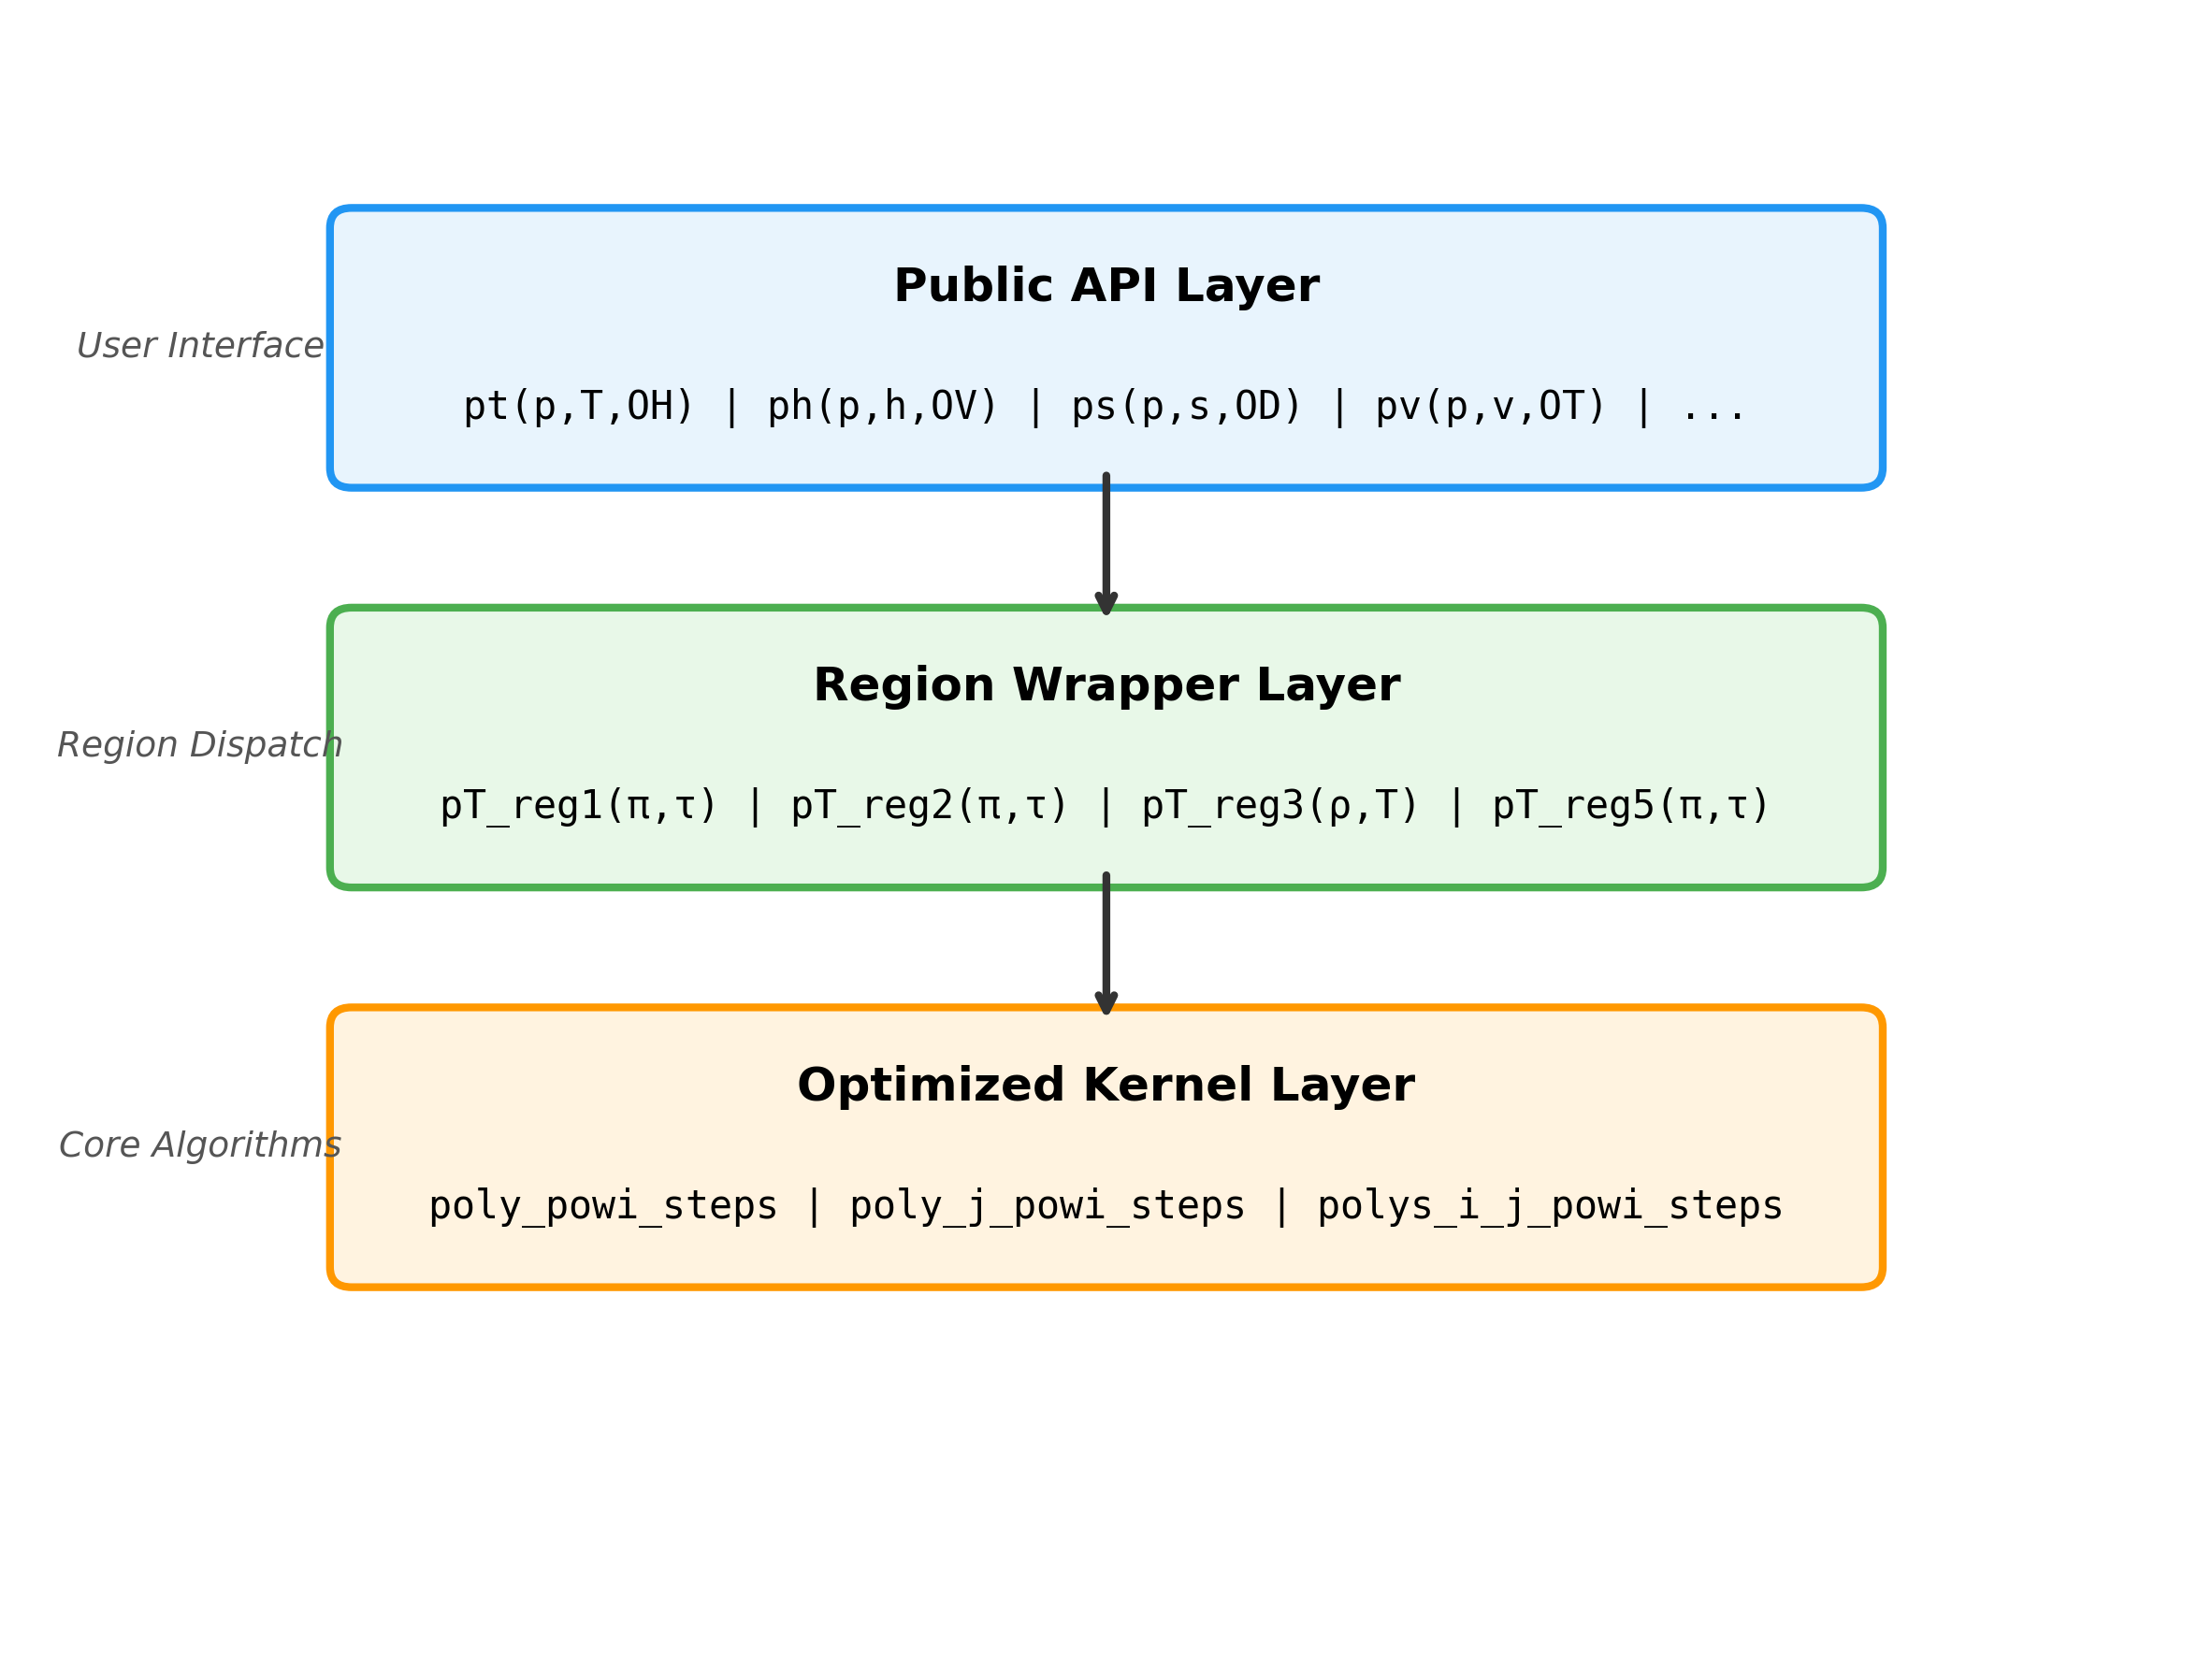
\includegraphics[width=0.9\textwidth]{architecture.png}
\caption{Three-layer architecture of SEUIF97}
\label{fig:architecture}
\end{figure}

SEUIF97 supports 12 input parameter pairs: $(p,t)$, $(p,h)$, $(p,s)$, $(p,v)$, $(t,h)$, $(t,s)$, $(t,v)$, $(h,s)$, $(p,x)$, $(t,x)$, $(h,x)$, $(s,x)$, and computes 36 thermodynamic, transport, and derived properties, including basic properties ($p$, $t$, $\rho$, $v$, $h$, $s$, $u$), derived properties ($c_p$, $c_v$, $w$, Helmholtz/Gibbs free energy, compressibility factor), partial derivatives, and transport properties ($\mu$, $\lambda$, $\sigma$).

To facilitate integration into diverse software ecosystems, SEUIF97 is publicly available as a Rust crate on crates.io, a Python package on PyPI, a WebAssembly package on npm, and with C bindings for broad compatibility. The source code is available at \texttt{https://github.com/thermalogic/RustSEUIF97} under the MIT license.

\section{Conclusions}

This paper proposed two acceleration techniques for the IAPWS-IF97 formula evaluation: recurrence polynomial-derivative computation and loop tiling. The key insight is that the IF97 fundamental equations and their partial derivatives share the same polynomial base terms, enabling simultaneous computation in a single pass. Combined with loop tiling for cache optimization, the proposed approach achieves 5x to 20x speedups over direct formula-based implementations, with the largest improvements in Regions 1 and 2 where the polynomial forms are most complex. These results demonstrate that directly accelerating the IAPWS-IF97 formulas can achieve competitive performance without resorting to approximation-based methods such as TTSE and SBTL. The Rust-based software package SEUIF97, available in multiple package formats, provides convenience for developers working in different programming environments.

\begin{thebibliography}{99}

\bibitem{IAPWS-IF97}
IAPWS, ``R7-97(2012): Revised Release on the IAPWS Industrial Formulation 1997 for the Thermodynamic Properties of Water and Steam,'' International Association for the Properties of Water and Steam, 2012. (The revision only relates to the extension of region 5 to 50 MPa) (August 2007).

\bibitem{Wagner2008}
W. Wagner, H.-J. Kretzschmar, ``International Steam Tables: Properties of Water and Steam Based on the Industrial Formulation IAPWS-IF97,'' 2nd ed., Springer, Berlin, 2008.

\bibitem{TTSE}
IAPWS, ``Release on the Tabular Taylor Series Expansion (TTSE) Method for the Calculation of Thermodynamic Properties of Water and Steam,'' International Association for the Properties of Water and Steam, 1997.

\bibitem{SBTL}
IAPWS, ``Release on the Spline-Based Table Lookup (SBTL) Method for the Calculation of Thermodynamic Properties of Water and Steam,'' International Association for the Properties of Water and Steam, 2015.

\bibitem{FreeSteam}
P. Colby, ``freeSteam: A C library for water/steam properties,'' https://sourceforge.net/projects/freesteam/.

\bibitem{IAPWS-Supplementary}
IAPWS, ``Release on the IAPWS Formulation 2008 for the Viscosity of Ordinary Water Substance,'' International Association for the Properties of Water and Steam, 2008.

\bibitem{LoopTiling}
M.E. Wolf, M.S. Lam, ``A data locality optimizing algorithm,'' Proceedings of the ACM SIGPLAN Conference on Programming Language Design and Implementation, 1991, pp. 30-44.

\bibitem{Criterion}
J. Boucher, ``Criterion.rs: Statistics-driven micro-benchmarking in Rust,'' https://github.com/bheisler/criterion.rs.

\end{thebibliography}

\end{document}
